\documentclass[aps,pre,twocolumn,superscriptaddress,nofootinbib]{revtex4-2}
\usepackage{graphicx}
\usepackage{amsmath,amssymb}
\usepackage{hyperref}

\begin{document}

\title{Arithmetic rigidity protects directed percolation:\\ squarefree versus shuffled quenched disorder}

\author{Davis Brief}
\email{davis@team8.co}
\affiliation{Team8 LLC, New York, NY, USA}

\date{June 11, 2026}

\begin{abstract}
We study $1{+}1$-dimensional directed site percolation in which a fixed fraction
($1-6/\pi^2 \approx 39.2\%$) of columns are weakened by a factor $c=0.6$, and compare two
arrangements of the same weak-column multiset: weak columns at the non-squarefree integers,
and the same columns randomly shuffled. The two systems differ only in the spatial order of
the disorder. We find that they behave differently in every respect measured. The critical
point shifts from $p_c=0.8207(1)$ (squarefree) to $p_c=0.8455(5)$ (shuffled). At criticality
the squarefree system shows a stable power-law density decay with exponent
$\alpha=0.155(15)$ over five decades, consistent with the clean directed percolation value
$\alpha \approx 0.1595$, while the shuffled system shows no stable power law anywhere in its
critical region: the effective exponent starts near $0.10$ and drifts monotonically toward
zero, the phenomenology expected from rare-region dominated, activated dynamics. We trace
the difference to the rigidity of the squarefree sequence: its weak-site runs are sharply
capped (longest run 8 in windows of $10^6$, versus 19 with an exponential tail when
shuffled), so the Griffiths regions that destabilize the disordered system are absent, and
its wandering exponent is $\omega \approx 1/4$ versus $1/2$ for the shuffle. The naive
Harris--Luck analysis would classify both disorders as relevant; up to $t=10^6$ the
squarefree system shows no sign of this. All headline results were reproduced by two
independent implementations written by agents given only the model definition, with no
information about the hypothesis or expected values.
\end{abstract}

\maketitle

\section{Introduction}

The directed percolation (DP) universality class is the canonical description of absorbing-state
phase transitions \cite{Hinrichsen2000,Janssen1981,Grassberger1982}. Its critical exponents,
e.g.\ the density-decay exponent $\alpha = \beta/\nu_\parallel \approx 0.159464$ in $1{+}1$
dimensions \cite{Jensen1999}, are shared by an enormous variety of models. The class is,
however, famously fragile to quenched spatial disorder: the Harris criterion
\cite{Harris1974} is violated in $d=1$ ($d\nu_\perp \approx 1.097 < 2$), and uncorrelated
disorder drives the transition to an infinite-randomness fixed point with activated dynamical
scaling, logarithmically slow decay, and Griffiths singularities
\cite{Hooyberghs2003,Vojta2006}.

For deterministic aperiodic modulations the corresponding relevance criterion is due to Luck
\cite{Luck1993}: a sequence whose cumulative fluctuations in a window of length $\ell$ grow
as $\ell^{\omega}$ is relevant when $\omega$ exceeds
$\omega_c = 1 - 1/(d\nu_\perp) \approx 0.089$. This framework has been explored for
substitution sequences such as Fibonacci and its generalizations
\cite{BarghathiNozadzeVojta2014}, where weak (small-$\omega$) modulations leave DP intact
and strong ones produce exotic infinite-modulation criticality.

Genuinely number-theoretic sequences have, to our knowledge, never been used as the disorder
in an absorbing-state transition, although their unusual statistical character is well
documented in the aperiodic-order literature: the squarefree integers (integers not divisible
by any perfect square) have density $6/\pi^2$, pure-point diffraction, and positive
topological entropy \cite{BaakeMoodyPleasants2000,Sarnak2011}. They sit in an interesting
middle ground: locally they pass many randomness tests (positive entropy), but globally they
are rigid, with maximal gaps that grow only like a small power of the position
\cite{FilasetaTrifonov1992} and sub-Poissonian count fluctuations in short intervals
\cite{Hall1982}. A positive-entropy sequence might be expected to act like random (Harris)
disorder; a rigid one might not. Which property controls the physics is not obvious, and we
are not aware of a prediction.

Here we settle the question numerically with a twin-control design. We place weak columns at
the non-squarefree positions, and compare against the \emph{identical multiset} of weak
columns placed at uniformly shuffled positions. Any difference between the two systems is
attributable purely to the arithmetic arrangement. We find that the difference is large and
qualitative.

\section{Model, observables, and verification protocol}

\subsection{Model}

We use directed site percolation on the tilted square lattice, written as a synchronous
stochastic cellular automaton. Site $i \in \{0,\dots,L-1\}$ (periodic) carries
$s_i(t)\in\{0,1\}$, and
\begin{equation}
s_i(t{+}1)=
\begin{cases}
1 & \text{w.p. } p_i \text{ if } s_i(t)=1 \text{ or } s_{i+1}(t)=1,\\
0 & \text{otherwise,}
\end{cases}
\label{eq:model}
\end{equation}
with independent draws per site and step. The clean model, $p_i = p$, has
$p_c = 0.705485$ \cite{Jensen1999}, which we use as a validation target. Quenched columnar
disorder enters through
\begin{equation}
p_i = \begin{cases} p & \text{site } i \text{ strong},\\ c\,p & \text{site } i \text{ weak},\end{cases}
\qquad c = 0.6 .
\end{equation}

Two disorder constructions are compared.
\emph{Squarefree:} site $i$ is strong iff $n_i = \mathrm{OFFSET} + i$ is squarefree.
\emph{Shuffled:} the strong/weak mask of the squarefree construction (same OFFSET, same $L$)
is randomly permuted. The weak fraction is $1-6/\pi^2 = 0.39207\ldots$ in both cases, exactly
matched sample by sample; only the ordering differs.

Runs start from the fully active state and record the density $\rho(t)$ at logarithmically
spaced times. The primary diagnostic is the local slope
$\alpha_{\rm eff}(t) = -\,d\ln\rho / d\ln t$, measured by least squares in sliding windows of
$\pm 0.6$ in $\ln t$. At a clean critical point $\alpha_{\rm eff} \to \alpha$; at an
infinite-randomness critical point $\rho \sim (\ln t)^{-x}$ and $\alpha_{\rm eff} \to 0$.

Production runs use $L=2^{20}$, $t \le 10^6$, and four disorder samples
(OFFSETs $10^6{+}3$, $5\times 10^7{+}17$, $3.6\times 10^8{+}1$, $9\times 10^8{+}7$, with
independent shuffle seeds for the control) per parameter point, simulated with an
independently written C engine (xoshiro256++ RNG) that was cross-validated against a separate
NumPy implementation on both the clean and disordered models (agreement within sampling error,
$\le 0.4\%$ in $\rho$ at $t=3\times 10^4$).

\subsection{Blind replication}

Because effective-exponent analyses are vulnerable to confirmation bias, the headline
measurements were replicated under a blinding protocol. Two additional implementations were
written from scratch by agents that received only the model definition of
Eq.~(\ref{eq:model}), the two disorder constructions, and a single directive: locate the
critical point of each construction in a stated bracket and characterize the long-time decay
as stable power law versus drifting. They received no information about the hypothesis, the
expected exponents, or each other, and they chose their own OFFSETs, RNG schemes, lattice
sizes ($L=2^{17}$), and analysis pipelines. Their results are quoted alongside ours in
Table~\ref{tab:results}. We regard this as the computational analogue of an independent
replication, and recommend the practice.

\begin{table}[t]
\caption{\label{tab:results}The same physics measured by three independent implementations.
Implementation 1 is this work's C engine ($L=2^{20}$, $t\le 10^6$, $n=4$ samples per point,
2 at the final bisection); implementations 2 and 3 are the blind replications
($L=2^{17}$, $t \le 10^6$, $n=3$--$4$). Quoted uncertainties are jackknife (impl.~2) or
spread over samples and bracketing (impl.~1).}
\begin{ruledtabular}
\begin{tabular}{lccc}
 & impl.~1 & impl.~2 (blind) & impl.~3 (blind) \\
\hline
$p_c$ squarefree & 0.8207(1) & 0.8207(3) & 0.8206--0.8208 \\
$p_c$ shuffled & 0.846--0.848 & 0.8455(5) & $\approx 0.8455$ \\
$\alpha$ squarefree & 0.155(15) & 0.18(3) & 0.15--0.19 \\
shuffled $\alpha_{\rm eff}$ drift & $0.10 \to 0.01$ & $0.108 \to 0.063$ & $0.07$--$0.10$, no plateau \\
\end{tabular}
\end{ruledtabular}
\end{table}

\section{Results}

\subsection{The critical point moves}

Bisection of the supercritical/subcritical boundary gives $p_c = 0.8207(1)$ for the
squarefree arrangement and $p_c$ between $0.845$ and $0.848$ (blind impl.~2: $0.8455(5)$)
for the shuffled control, a shift $\Delta p_c \approx 0.025$ at identical composition. The
squarefree arrangement is the more efficient spreader: its weak sites never cluster into the
long blocking segments that the shuffle produces, so less infection strength is needed to
percolate. The shift itself is a non-universal quantity, but its size, roughly $3\%$ of
$p_c$ from pure rearrangement, is a first indication that ordering matters strongly here.

\subsection{Critical decay: stable power law versus drift}

\begin{figure}[t]
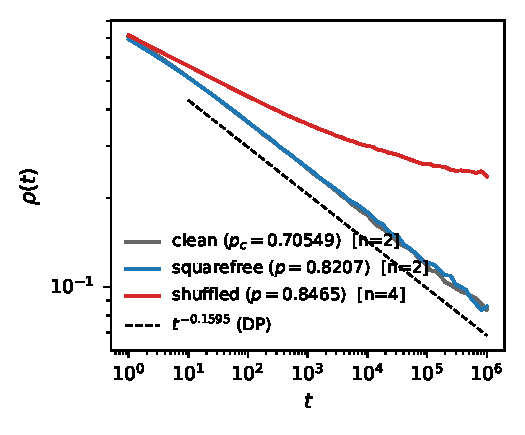
\includegraphics[width=\columnwidth]{fig1_rho.pdf}
\caption{\label{fig:rho}Density decay from a fully active start at the respective critical
points: clean control at $p_c=0.705485$, squarefree at $p=0.8207$, shuffled at $p=0.8465$
(averages over samples; $L=2^{20}$). The dashed guide is the clean DP law
$t^{-0.1595}$.}
\end{figure}

\begin{figure}[t]
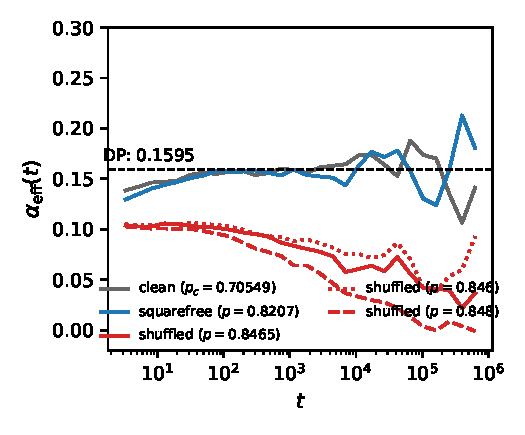
\includegraphics[width=\columnwidth]{fig2_alpha.pdf}
\caption{\label{fig:alpha}Local slope $\alpha_{\rm eff}(t)$ for the curves of
Fig.~\ref{fig:rho}, plus the shuffled control at two additional couplings spanning its
critical bracket. The clean and squarefree systems sit on the DP value (dashed) for the
full accessible range; the shuffled system starts near $0.10$ and drifts monotonically
toward zero at every coupling in its bracket. Late-time scatter in the clean and squarefree
curves reflects the small number of samples ($n=2$) at the final bisection point.}
\end{figure}

Figures~\ref{fig:rho} and \ref{fig:alpha} contain the central result. At its critical point
the squarefree system is indistinguishable from the clean system: $\alpha_{\rm eff}$ rises to
the DP value by $t \approx 10^2$ and stays there to $t = 10^6$, with
$\alpha = 0.155(15)$ from the production data. The blind replication (impl.~2) fitted a
single power law with $\alpha = 0.18(3)$ over $t\in[10^3,10^6]$ and found the power-law form
to fit decisively better than a logarithmic form (RMS residual $0.035$ versus $0.059$),
with no drift of $\alpha_{\rm eff}$ toward zero.

The shuffled control never produces a power law. Across five couplings spanning its critical
bracket ($p = 0.845$ to $0.850$), $\alpha_{\rm eff}$ begins near $0.10$, well below the DP
value, and decreases monotonically with time (Fig.~\ref{fig:alpha}); on the subcritical side
it instead turns sharply upward (peel-off). At no coupling does a plateau form. The blind
replication additionally reports strong sample-to-sample heterogeneity near criticality
($\rho(10^6)$ ranging over a factor of two at fixed coupling) and finds power-law and
$(\ln t)^{-x}$ fits comparably mediocre, with $x \approx 1$. This is the standard
phenomenology of a disordered absorbing-state transition governed by rare regions
\cite{Hooyberghs2003,Vojta2006}. We deliberately make only the conservative claim supported
at $t \le 10^6$: the shuffled system has no stable power law and drifts in the activated
direction, while its arithmetic twin holds the clean DP exponent over the same range with
the same statistics.

\subsection{Mechanism: rare-region starvation and rigidity}

\begin{figure}[t]
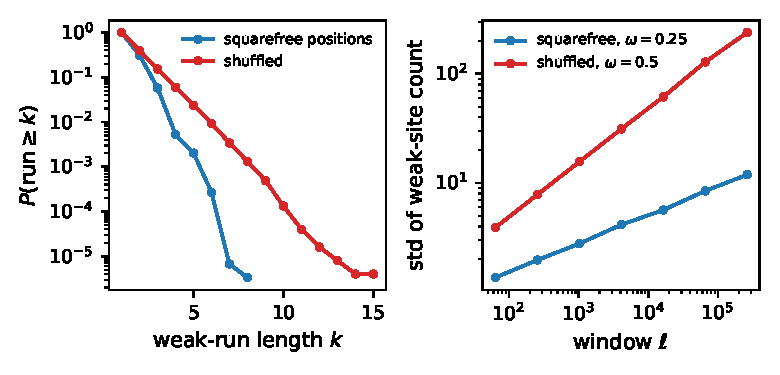
\includegraphics[width=\columnwidth]{fig3_disorder.pdf}
\caption{\label{fig:disorder}Statistics of the two disorder arrangements at identical
composition ($L=2^{20}$ window, OFFSET $10^6{+}3$). Left: survival function of weak-run
lengths. The shuffle has the geometric tail of Bernoulli disorder (runs up to 19 observed);
the squarefree arrangement is capped at run length 8. Right: standard deviation of the
weak-site count in windows of length $\ell$, giving wandering exponents
$\omega \approx 0.25$ (squarefree) versus $\omega = 0.5$ (shuffled).}
\end{figure}

The microscopic origin of the difference is visible directly in the disorder statistics
(Fig.~\ref{fig:disorder}). Long runs of consecutive weak sites are the locally subcritical
inclusions whose exponentially long lifetimes generate Griffiths physics and, at
criticality, activated scaling \cite{Vojta2006}. In the shuffled arrangement weak-run
lengths are geometric with ratio $0.392$, with runs up to 19 in a window
of $10^6$. In the squarefree arrangement a run of $k$ consecutive non-squarefree integers
requires $k$ distinct square divisors in $k$ consecutive integers; runs are capped at 8 in
all windows used ($P(\mathrm{run}\ge 5)$ is twelve times smaller than for the shuffle), and
the maximal gap between squarefree numbers grows only like a small power
\cite{FilasetaTrifonov1992}. The squarefree system simply has no rare regions worth the
name: number theory removes the tail.

The same rigidity appears at large scales as hyperuniform-like suppression of fluctuations:
the measured wandering exponent is $\omega = 0.252$ (theory: window-count variance
$\propto \ell^{1/2}$ \cite{Hall1982}, hence $\omega = 1/4$), versus $\omega = 1/2$ for the
shuffle. This places the result in interesting tension with the Harris--Luck framework.
With $\omega = 1/4 > \omega_c \approx 0.089$, a naive application of the Luck criterion
classifies even the squarefree arrangement as relevant, yet no departure from DP is visible
up to $t=10^6$, while the $\omega = 1/2$ twin departs immediately and dramatically. Either
the asymptotic crossover for the rigid arrangement lies beyond accessible scales because the
relevant amplitude (set by the rare-region content, not only by $\omega$) is tiny, or the
Luck classification, derived for bounded-fluctuation substitution sequences, does not
transfer directly to positive-entropy rigid sequences. We consider distinguishing these two
readings the main theoretical question raised by this work. A related mechanism is known
from topologically disordered lattices, where anticorrelations of coordination numbers
suppress the disorder relevant at the Harris level \cite{BarghathiVojta2014}, and from
hyperuniform point sets generally \cite{TorquatoStillinger2003}; the squarefree integers
provide a deterministic, maximally reproducible instance with $\omega$ strictly between the
periodic and random values.

\section{Discussion}

The twin-control design gives the result an unusual degree of internal protection: both
systems share the same update rule, the same weak-site multiset, the same engines, the same
analysis, and the same time horizon, so none of these can explain the difference. What
remains is the arithmetic arrangement. In this sense the absorbing-state transition acts as
a physical detector of the multiplicative structure of the integers: it distinguishes the
squarefree sequence from its own shuffle through universality-class phenomenology, not
through any density measurement.

Limitations. First, $t = 10^6$ and $L = 2^{20}$ cannot exclude an asymptotic crossover of
the squarefree system away from DP; our claim is the equal-time, equal-statistics contrast,
not infinite-time universality. Second, we studied one weakness factor ($c=0.6$) and one
observable class (density decay from full occupancy); spreading-from-seed exponents and the
$c$ dependence (the Luck amplitude grows as $c \to 0$) are natural next measurements. Third,
the critical-point uncertainty of the shuffled system is intrinsically larger because its
transition is smeared by sample heterogeneity; our conclusions about it are deliberately
qualitative (absence of a stable power law, direction of drift) rather than a fitted
$(\ln t)^{-x}$ exponent.

Extensions suggest themselves immediately: $k$-free integers interpolate the gap statistics;
the M\"obius function provides a three-valued disorder with conjectured maximal
pseudo-randomness \cite{Sarnak2011}; primes provide density-vanishing disorder; and temporal
(rather than spatial) arithmetic disorder probes the time-direction analogue. If the
protection observed here is controlled by the run-length cap, the $k$-free family should
show a systematic approach to random behavior as $k$ grows and the cap loosens.

\emph{Methods disclosure.} This work was performed with substantial use of AI research
assistants (Anthropic's Claude Fable 5 and Claude Opus 4.8 models), which carried out the simulations, implementations, and
drafting under the author's direction; the blind-replication protocol of
Sec.~II.B, in which independent implementations were produced by context-isolated agents,
was adopted specifically to guard against self-confirmation in an AI-assisted workflow. All
code (C and Python engines, analysis, and the blind-protocol specifications) and all raw
data are public at \url{https://github.com/adventurelands/squarefree-percolation}.

\begin{thebibliography}{99}

\bibitem{Hinrichsen2000} H. Hinrichsen, Adv. Phys. \textbf{49}, 815 (2000).

\bibitem{Janssen1981} H. K. Janssen, Z. Phys. B \textbf{42}, 151 (1981).

\bibitem{Grassberger1982} P. Grassberger, Z. Phys. B \textbf{47}, 365 (1982).

\bibitem{Jensen1999} I. Jensen, J. Phys. A \textbf{32}, 5233 (1999).

\bibitem{Harris1974} A. B. Harris, J. Phys. C \textbf{7}, 1671 (1974).

\bibitem{Hooyberghs2003} J. Hooyberghs, F. Igl\'oi, and C. Vanderzande, Phys. Rev. Lett.
\textbf{90}, 100601 (2003).

\bibitem{Vojta2006} T. Vojta, J. Phys. A \textbf{39}, R143 (2006).

\bibitem{Luck1993} J. M. Luck, Europhys. Lett. \textbf{24}, 359 (1993).

\bibitem{BarghathiNozadzeVojta2014} H. Barghathi, D. Nozadze, and T. Vojta, Phys. Rev. E
\textbf{89}, 012112 (2014).

\bibitem{BaakeMoodyPleasants2000} M. Baake, R. V. Moody, and P. A. B. Pleasants, Discrete
Math. \textbf{221}, 3 (2000).

\bibitem{Sarnak2011} P. Sarnak, \emph{Three lectures on the M\"obius function, randomness
and dynamics}, lecture notes, Institute for Advanced Study (2011).

\bibitem{FilasetaTrifonov1992} M. Filaseta and O. Trifonov, J. London Math. Soc.
\textbf{45}, 215 (1992).

\bibitem{Hall1982} R. R. Hall, Mathematika \textbf{29}, 7 (1982).

\bibitem{BarghathiVojta2014} H. Barghathi and T. Vojta, Phys. Rev. Lett. \textbf{113},
120602 (2014).

\bibitem{TorquatoStillinger2003} S. Torquato and F. H. Stillinger, Phys. Rev. E
\textbf{68}, 041113 (2003).

\end{thebibliography}

\end{document}
